\documentclass{article}

\usepackage{mathrsfs,amsmath}
\usepackage{xcolor}
\usepackage{titlesec}
\usepackage{listings}
\usepackage{syntax}
\usepackage{pythonhighlighting}
\usepackage{fancyvrb}

\usepackage{graphicx}

\graphicspath{ {./assets/} }

\usepackage[margin=1.4in]{geometry}

\title{Homework \#2 | Fall 2021} 
\author{Jared Dyreson\\ 
        California State University, Fullerton}

\DeclareRobustCommand{\bowtie}{%
  \mathrel\triangleright\joinrel\mathrel\triangleleft}


\usepackage [english]{babel}
\usepackage [autostyle, english = american]{csquotes}
\MakeOuterQuote{"}

\titlespacing*{\section}
{0pt}{5.5ex plus 1ex minus .2ex}{4.3ex plus .2ex}
\titlespacing*{\subsection}
{0pt}{5.5ex plus 1ex minus .2ex}{4.3ex plus .2ex}

\usepackage{hyperref}
\hypersetup{
    colorlinks,
    citecolor=black,
    filecolor=black,
    linkcolor=black,
    urlcolor=black
}

\begin{document}

\maketitle
\tableofcontents

\newpage


\section{Questions}

\begin{enumerate}

\item Brute force password guessing. Each of the following are a different kind of password. An attacker can always try to bypass password security by guessing every possible password that might exist. In the worst case  (for the attacker), the correct password is the last one that they guess. So increasing the number of potential passwords makes password protection more effective. For each password type, \textbf{compute the number of passwords of that type exist.} Justify your answers

\begin{itemize}
\item \textbf{Eight lower-case letters, upper-case letters, or digits}: There are 26 letters in the English alphabet, which have both upper and lower case. Therefore in any given slot, there could be 52 different possibilities. Also there are 10 individual digits that we can use as well. This will bring our total to 62. To get all the possible permutations of a given for a string of length 8 would be $62^{8}$ passwords.
\item \textbf{Nine letters:} In this instance, we are not told if each letter is upper or lower case or a combination of the two. For this, we will calculate both. Strictly upper/lower case (AAAAAAAAAA || aaaaaaaaa): $26^{9}$. If we have a mixture of the two (AAAAaaaaA): $52^{9}$
\end{itemize}
\item Give the definitions for the three distinct functions: $g_{1}(n), g_{2}(n), g_{3}(n)$ that are members in the set $O(n^{3})$

\begin{itemize}
\item $g_{1}(n) = 10n^{2}$
\item $g_{2}(n) = n\log(n)$
\item $g_{3}(n) = 100n^{3} + 20n^{2} + 100n + 69$
\end{itemize}
\item Evaluate each of the following complexity functions for: $n = 2^{3} = 8$ , $n = 2^{7} = 128$, $n = 2^{10} = 1024$

\begin{itemize}
\item $\log_{2}(n)$
\item $n$
\item $n^{2}$
\item $n^{3}$
\item $2^{n}$
\item $n!$
\end{itemize}

\begin{table}[!h]
\centering
\begin{tabular}{|l|l|l|l|}
\hline
 & $n = 2^{3}$ & $n = 2^{7}$ & $n = 2^{10}$ \\ \hline
$log_{2}(n)$ & 3 & 7 & 10 \\ \hline
$n$ & 8 & 128 & 1024 \\ \hline
$n^{2}$ & 64 & 16384 & 1048576 \\ \hline
$n^{3}$ & 512 & 2097152 & 1073741824 \\ \hline
$2^{n}$ & 256 & $3.4028 \times 10^{38}$ & MATH ERROR \\ \hline
$n!$ & 40320 & MATH ERROR & MATH ERROR \\ \hline
\end{tabular}
\end{table}

\newpage

\item The diagram above represents a graph. Use the following abbreviations to represent the nodes: MH= Mayors house; BA= Bakery; MF= McFanes’s Farm; BR= Brewery; TF= Thomas’ Farm; IN=In; DC= Dry cleaner; LI=Library and CH= City Hall

\begin{itemize}
\item Time complexity for adding connection: $O(1)$. If you have both indices, the lookup can be done in constant time.
\item Time complexity for removal: $O(E)$
\end{itemize}

\begin{table}[!h]
\centering
\begin{tabular}{|l|l|l|l|l|l|l|l|l|l|}
\hline
 & \textbf{MH} & \textbf{BA} & \textbf{MF} & \textbf{BR} & \textbf{TF} & \textbf{IN} & \textbf{DC} & \textbf{LI} & \textbf{CH} \\ \hline
\textbf{MH} & $\infty$ & $\infty$ & $\infty$ & $\infty$ & $\infty$ & $\infty$ & $\infty$ & $\infty$ & $\infty$ \\ \hline
\textbf{BA} & 17 & $\infty$ & $\infty$ & $\infty$ & $\infty$ & $\infty$ & $\infty$ & $\infty$ & $\infty$ \\ \hline
\textbf{MF} & $\infty$ & 9 & $\infty$ & 21 & 12 & $\infty$ & $\infty$ & $\infty$ & $\infty$ \\ \hline
\textbf{BR} & 17 & $\infty$ & $\infty$ & $\infty$ & $\infty$ & $\infty$ & $\infty$ & $\infty$ & $\infty$ \\ \hline
\textbf{TF} & $\infty$ & $\infty$ & 12 & $\infty$ & $\infty$ & $\infty$ & $\infty$ & $\infty$ & $\infty$ \\ \hline
\textbf{IN} & $\infty$ & $\infty$ & $\infty$ & 5 & $\infty$ & $\infty$ & $\infty$ & $\infty$ & $\infty$ \\ \hline
\textbf{DC} & $\infty$ & $\infty$ & $\infty$ & $\infty$ & $\infty$ & 19 & $\infty$ & $\infty$ & 12 \\ \hline
\textbf{LI} & $\infty$ & $\infty$ & $\infty$ & $\infty$ & $\infty$ & 6 & $\infty$ & $\infty$ & 12 \\ \hline
\textbf{CH} & $\infty$ & $\infty$ & $\infty$ & $\infty$ & $\infty$ & $\infty$ & 12 & 12 & $\infty$ \\ \hline
\end{tabular}
\end{table}

\begin{itemize}
\begin{figure}[!h]
\centering
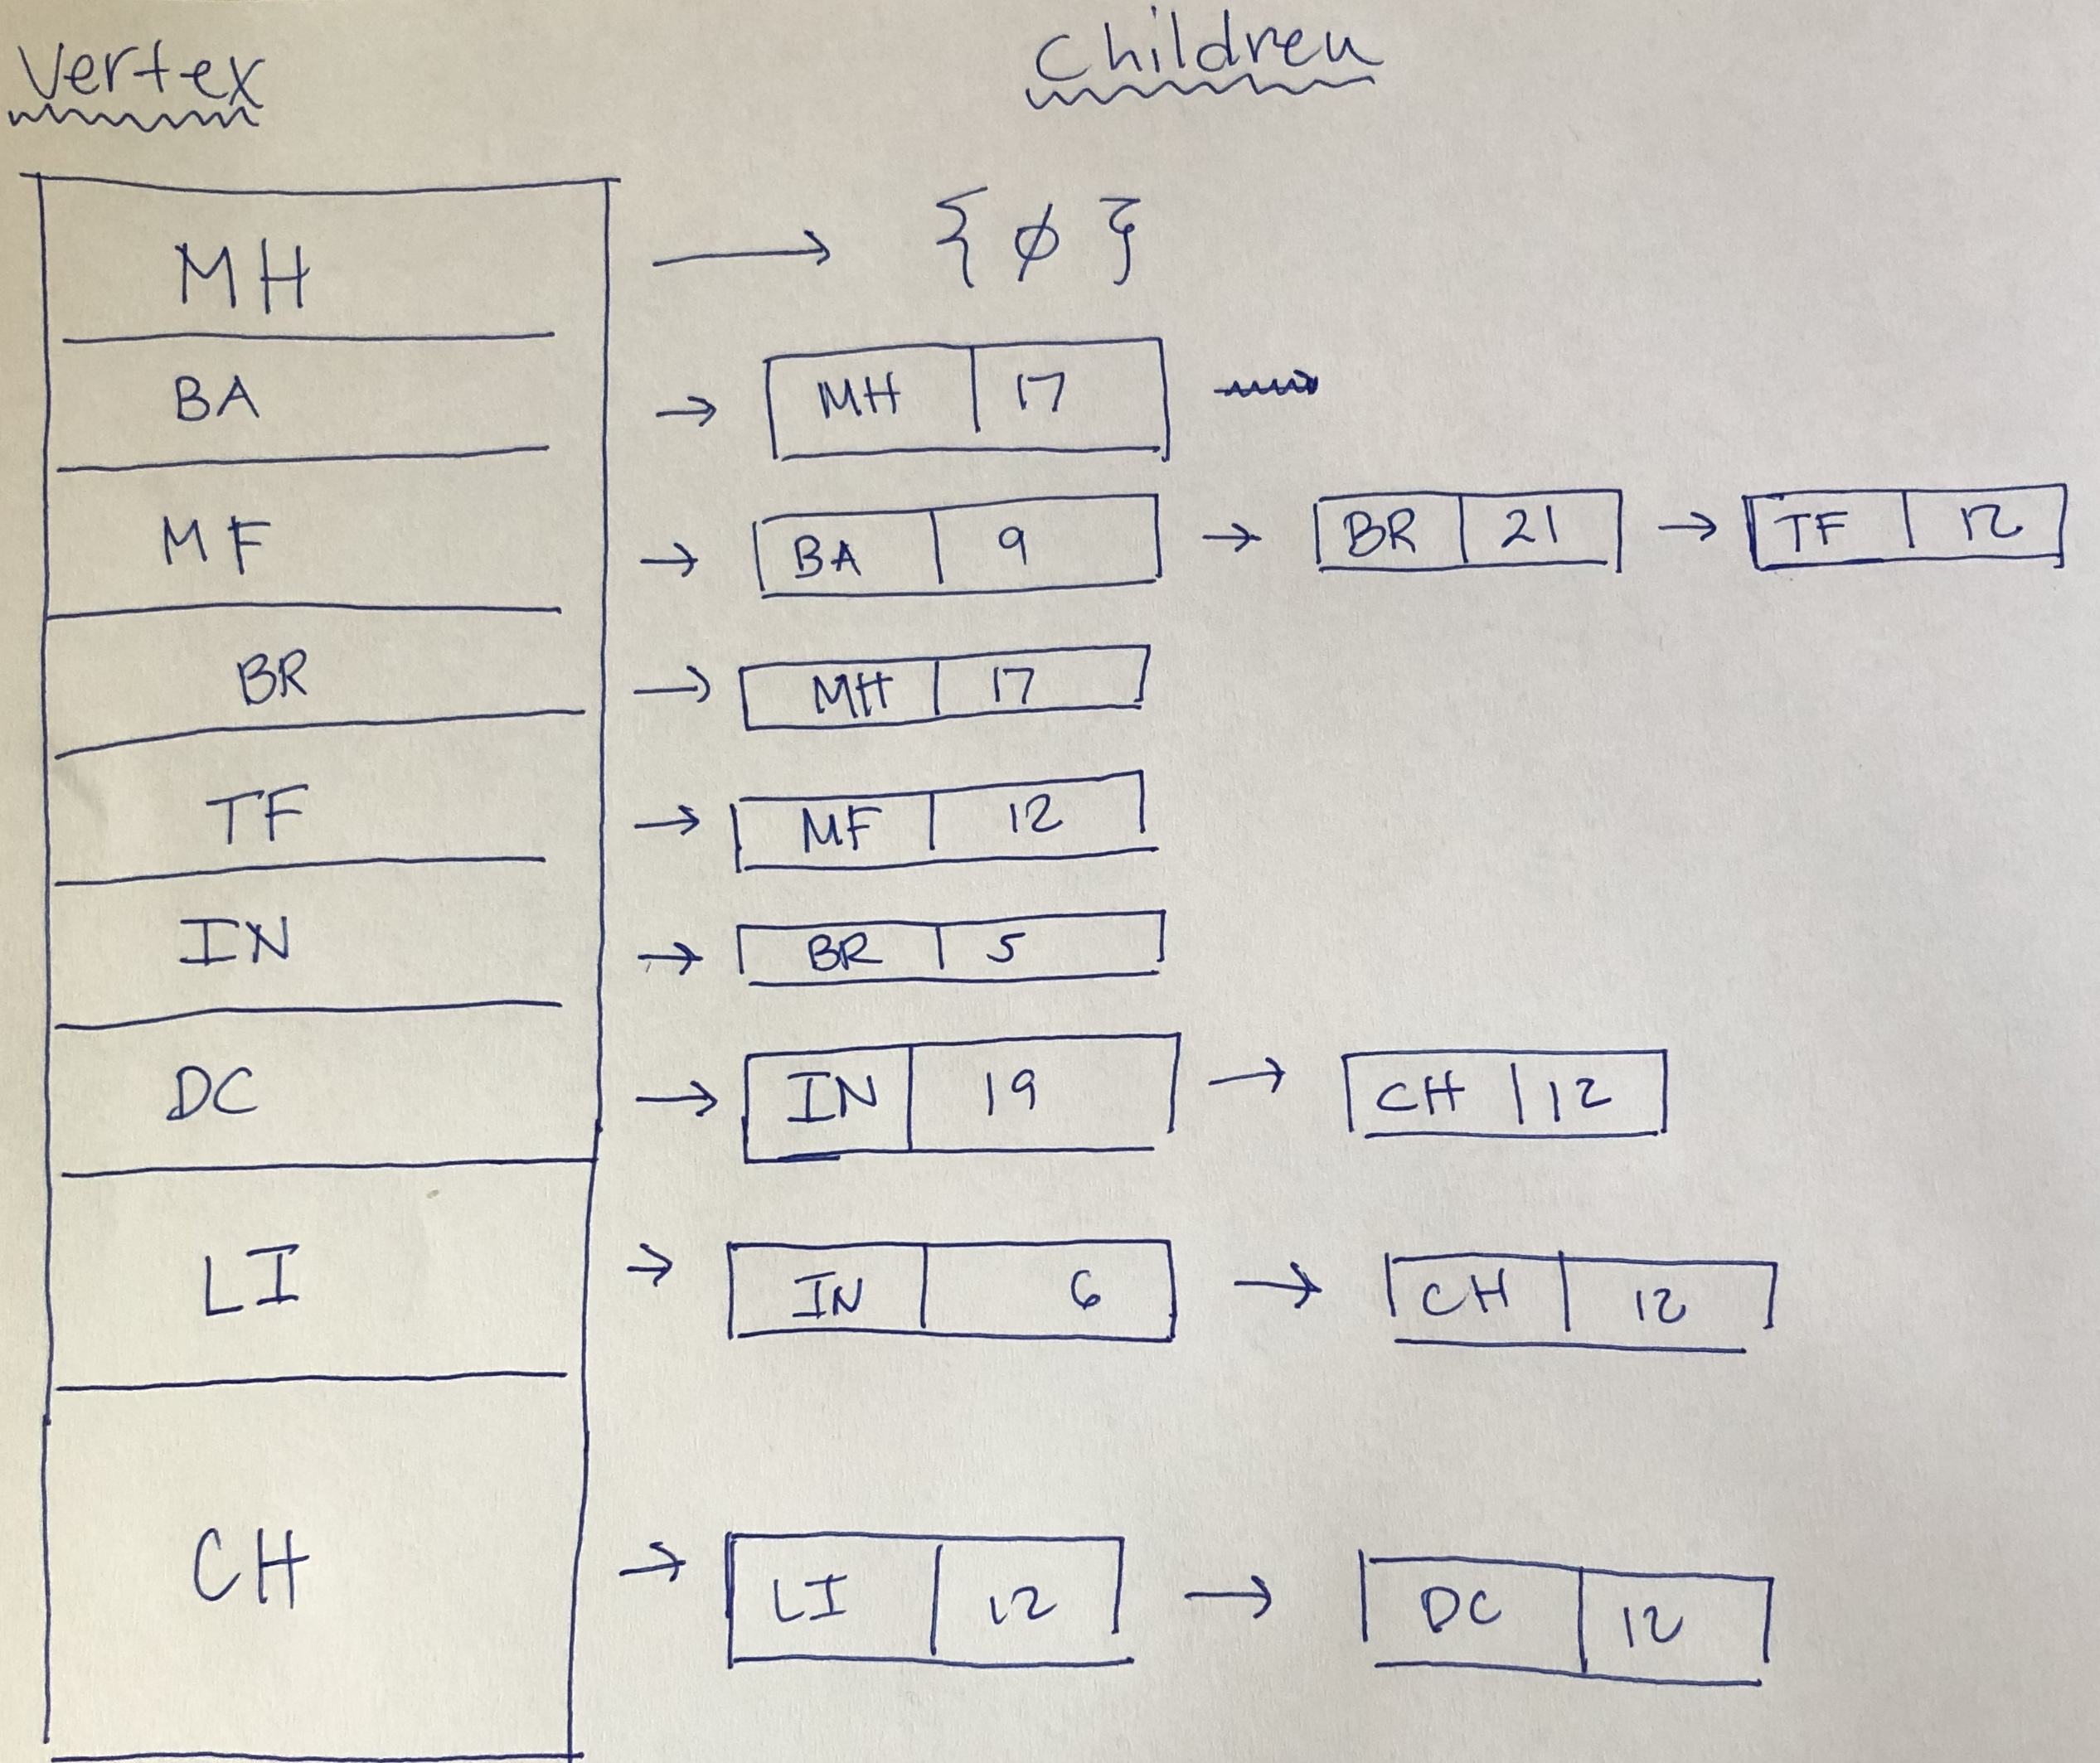
\includegraphics[width=10cm]{adjacency_list}
\caption{Adjacency List}
\end{figure}
\newpage
\item The maximal number for graph density is derived from this formula: \\
      $$M = \frac{|V|(|V|-1)}{2}$$ which can  be applied in this instance: \\
      $$M = \frac{9(9 - 1)}{2} \implies \frac{72}{2} \implies 36$$
\item The number of number of edges in our graph is only 10, therefore making it \textbf{sparse}.
\item Since none of our edges intersect one another, the graph is also \textbf{planar}.
\end{itemize}

\end{enumerate}

\end{document}

